\documentclass[10pt,xcolor=pdflatex,hyperref={unicode}]{beamer}
\usepackage{newcent}
\usepackage[utf8]{inputenc}
%\usepackage[czech]{babel}
%\usepackage[T1]{fontenc}
\usepackage{hyperref}
\usepackage{fancyvrb}
\usetheme{FIT}

\usepackage{setspace}
\usepackage{enumerate}
\usepackage[export]{adjustbox}
\usepackage{wrapfig}
%%%%%%%%%%%%%%%%%%%%%%%%%%%%%%%%%%%%%%%%%%%%%%%%%%%%%%%%%%%%%%%%%%
\title{Evaluating Reliability of \\ Static Analysis Results \\  Using Machine Learning}

\author[]{
Tomáš Beránek\\
\footnotesize{Supervisor: prof. Ing. Tomáš Vojnar, Ph.D.}\\
\footnotesize{Consultants: Ing. Viktor Malík, Mgr. Marek Grác, Ph.D.}
}

\institute[]{Brno University of Technology, Faculty of Information Technology}
%Bo\v{z}et\v{e}chova 1/2. 612 66 Brno - Kr\'alovo Pole\\
%login@fit.vutbr.cz}

%\institute[]{xberan46@stud.fit.vutbr.cz\\
%Fakulta informačních technologií Vysokého učení technického v Brně\\
%Bo\v{z}et\v{e}chova 1/2. 612 66 Brno - Kr\'alovo Pole\\
%}

% České logo - Czech logo
% beamerouterthemeFIT.sty řádek 9: fitlogo1_cz

\date{February 1, 2023}
%\date{\today}
%\date{} % bez data / without date

%%%%%%%%%%%%%%%%%%%%%%%%%%%%%%%%%%%%%%%%%%%%%%%%%%%%%%%%%%%%%%%%%%


\begin{document}


\frame[plain]{\titlepage}

\begin{frame}
  \frametitle{Motivation -- Meta Infer}
  \begin{columns}
    \column{0.6\textwidth}
    \doublespacing
    \begin{itemize}
        \item \large{Advantages}:
            \begin{itemize}
            \doublespacing
                \item highly \emph{scalable},
                \item easy to use,
                \item can analyze variety of software \\ (with a \emph{wrapper}).
                 \singlespacing
            \end{itemize}
        \item \large{Disadvantages}:
            \begin{itemize}
                \item too many False Positives (FP) \\ (\alert{almost 90 \%!}).
                \singlespacing
            \end{itemize}
    
    \end{itemize}
     
    \column{0.4\textwidth}
    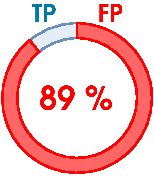
\includegraphics[width=0.9\textwidth]{img/fp-rate.pdf}
  \end{columns}
\end{frame} 


\begin{frame}\frametitle{Objectives of the Thesis}
\doublespacing
    \begin{itemize}
        \item \emph{Identify} false positives using \emph{deep learning}.
        \begin{itemize}
            \item Choose a suitable kind on NN:
            \begin{itemize}
                \item \emph{Graph Neural Network} (GNN).
            \end{itemize}
            \item Choose a suitable code representation:
            \begin{itemize}
                \item \emph{Code Property Graph} (CPG).
            \end{itemize}
        \end{itemize}
        \item \alert{Input}: source files and build scripts.
        \item \alert{Output}: probability of being FP for each reported issue.
    \end{itemize}
\end{frame}


\begin{frame}\frametitle{Proposed Solution}
\doublespacing
    \begin{itemize}
        \item The false positive detection system consists of:
        \begin{itemize}
            \item source code \emph{transformation},
            \item trained \emph{model}.
        \end{itemize}
    \end{itemize}
    \vspace{0.7cm}
    \begin{center}
        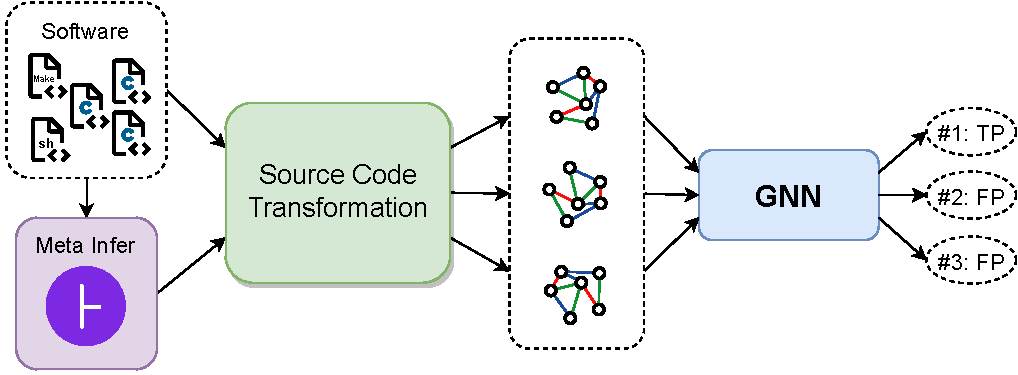
\includegraphics[width=0.95\textwidth]{img/overall.drawio.pdf}
    \end{center}

\end{frame}


\begin{frame}
\frametitle{Existing Approaches for Graph Construction}
\doublespacing

    \begin{itemize}
        \item Existing approaches often use \emph{Joern}.
        \item Disadvantages of existing approaches:
        \begin{itemize}
            \item not considering \emph{conditional compilation},
            \doublespacing
            \item inability to automatically identify required source files.
        \end{itemize}
        \item The proposed solution also has a slightly \emph{different use case}.
    \end{itemize}
\end{frame}


\begin{frame}\frametitle{Graph Construction Pipeline}
\doublespacing

    \begin{itemize}
    \item Input is limited to C and a subset of C++.
        \item The output CPG is neither language- nor analyzer-dependent.
        \item \alert{Input}: \emph{compilation commands} (source files).
        \item \alert{Output}: \emph{code property graph} for each reported issue.
    \end{itemize}
    \vspace{0.5cm}
    \hspace{-0.77cm}
    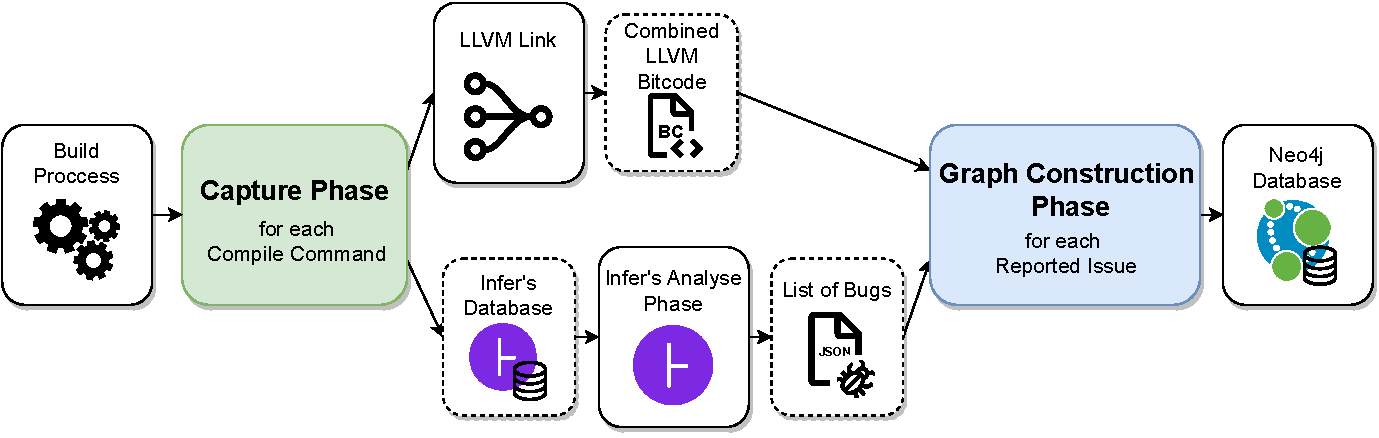
\includegraphics[width=1.13\textwidth]{img/all-modified.drawio.pdf}
\end{frame}


\begin{frame}\frametitle{Capture Phase}
\doublespacing
    \begin{itemize}
        \item \alert{Input}: \emph{compilation commands} (source files).
        \item \alert{Output}: combined \emph{LLVM bitcode} and a \emph{list of issues}.
    \end{itemize}
    \vspace{0.8cm}
    \hspace{-0.77cm}
    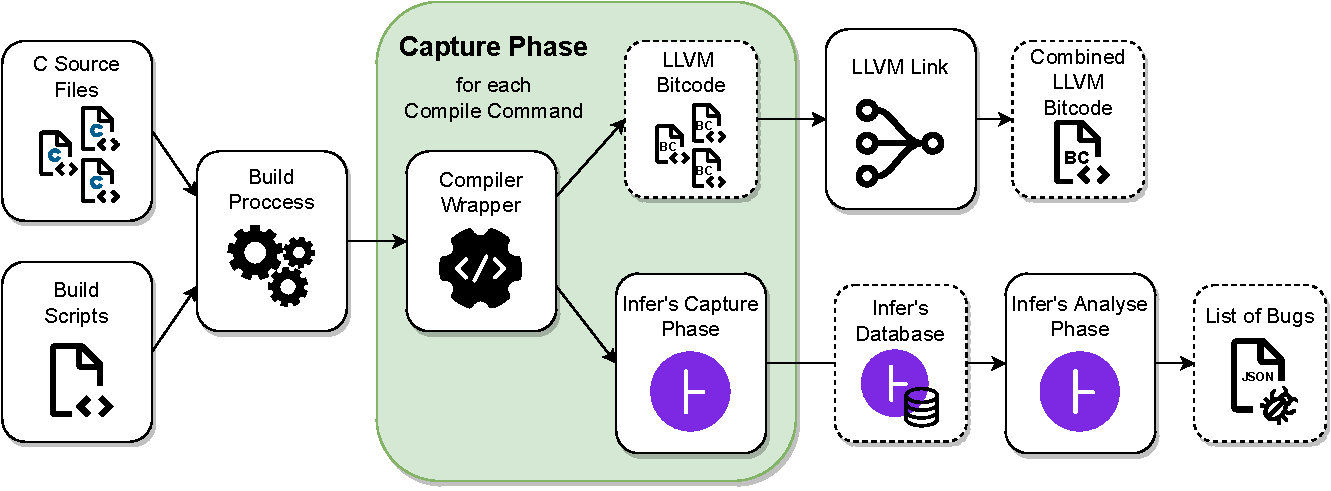
\includegraphics[width=1.13\textwidth]{img/capture-modified.drawio.pdf}
\singlespacing
\end{frame}


\begin{frame}\frametitle{Graph Construction Phase}
\doublespacing

    \begin{itemize}
        \item \alert{Input}: combined \emph{LLVM bitcode} and a \emph{list of issues}.
        \item \alert{Output}: \emph{code property graph} for each reported issue.
    \end{itemize}
    \vspace{0.8cm}
    \hspace{-0.77cm}
    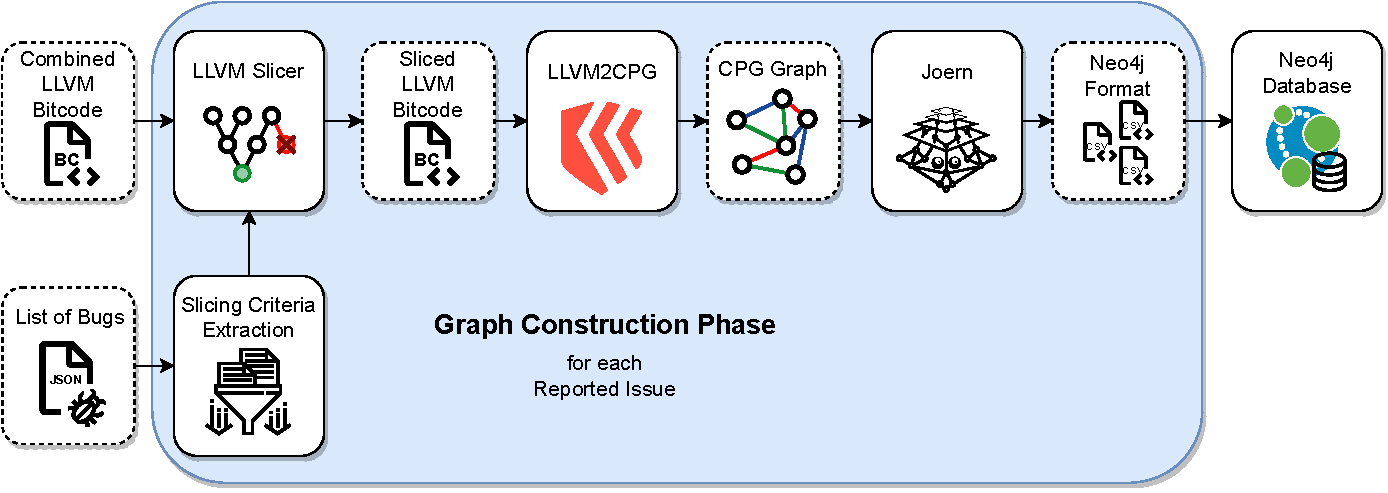
\includegraphics[width=1.13\textwidth]{img/construction-modified.drawio.pdf}
\singlespacing
\end{frame}

\begin{frame}\frametitle{Future Work}
\doublespacing

    \begin{enumerate}
        \item \emph{Automation} of the graph construction pipeline.
        \item Graph extraction from the \emph{D2A dataset}.
        \item \emph{GNN model architecture} selection and training.
        \item Implementation of \emph{self-training}.
        \item Integration with \emph{csmock}.
        \item Experiments on \emph{SRPM packages}.
    \end{enumerate}

\singlespacing
\end{frame}

\end{document}
